% <- percent signs are used to comment
\documentclass[12pt]{article}

%%%%%% PACKAGES - this part loads additional material for LaTeX %%%%%%%%%
% Nearly anything you want can be done in LaTeX if you load the right package 
% (search ctan.org or google it if you are looking for something).  We will load
% here a few that we need for this document or that we expect you to need later.

% The next 3 lines are needed to fix shortcomings of TeX that only make sense given its 40-year history ...
% Simple keep and ignore.
\usepackage[utf8]{inputenc}
\usepackage[T1]{fontenc}
\usepackage{lmodern}
\usepackage{amsmath}
\usepackage{changepage}
\usepackage{lipsum}
\usepackage{caption}

% Custom margins (and paper sizes etc.) because LaTeX else wastes much space
\usepackage[margin=1in]{geometry}

% The following packages are created by the American Mathematical Society (AMS)
% and provide lots of tools for special fonts, symbols, theorems, and proof
\usepackage{amsmath,amsfonts,amssymb,amsthm}
% mathtools contains many detail improvements over ams and core tex
\usepackage{mathtools}

% graphicx is required for images
\usepackage{graphicx}

% enumitem used for customizing enumerations
\usepackage[shortlabels]{enumitem}

% tikz is the package used for drawing, in particular for drawing trees. You may also find simplified packages like tikz-qtree and forest useful
\usepackage{tikz}

% hyperref allows links, urls, and many other PDF tricks.  We load it here
%          in such a way that the PDF file has info about it
\usepackage[%
	pdftitle={CS240 Assignment 0},%
	hidelinks,%
]{hyperref}


%%%%%% COMMANDS - here you can define your own LaTeX-commands %%%%%%%%%

%%%%%% End of Preamble %%%%%%%%%%%%%

\begin{document}

\begin{center}
{\Large\textbf{CS240, Spring 2022}}\\
\vspace{2mm}
{\Large\textbf{Assignment 5: Question 2}}\\
\vspace{3mm}
\end{center}

\begin{adjustwidth}{0em}{0pt}
\textbf{Q2a)} Trace the algorithm to build the Huffman trie for the string {\tt mississauga}, and name the result $T_1$. Repeat the process for the string {\tt massasauga}, and name the result $T_2$.\\\\
\begin{figure}[tbhp]
	\begin{center}
		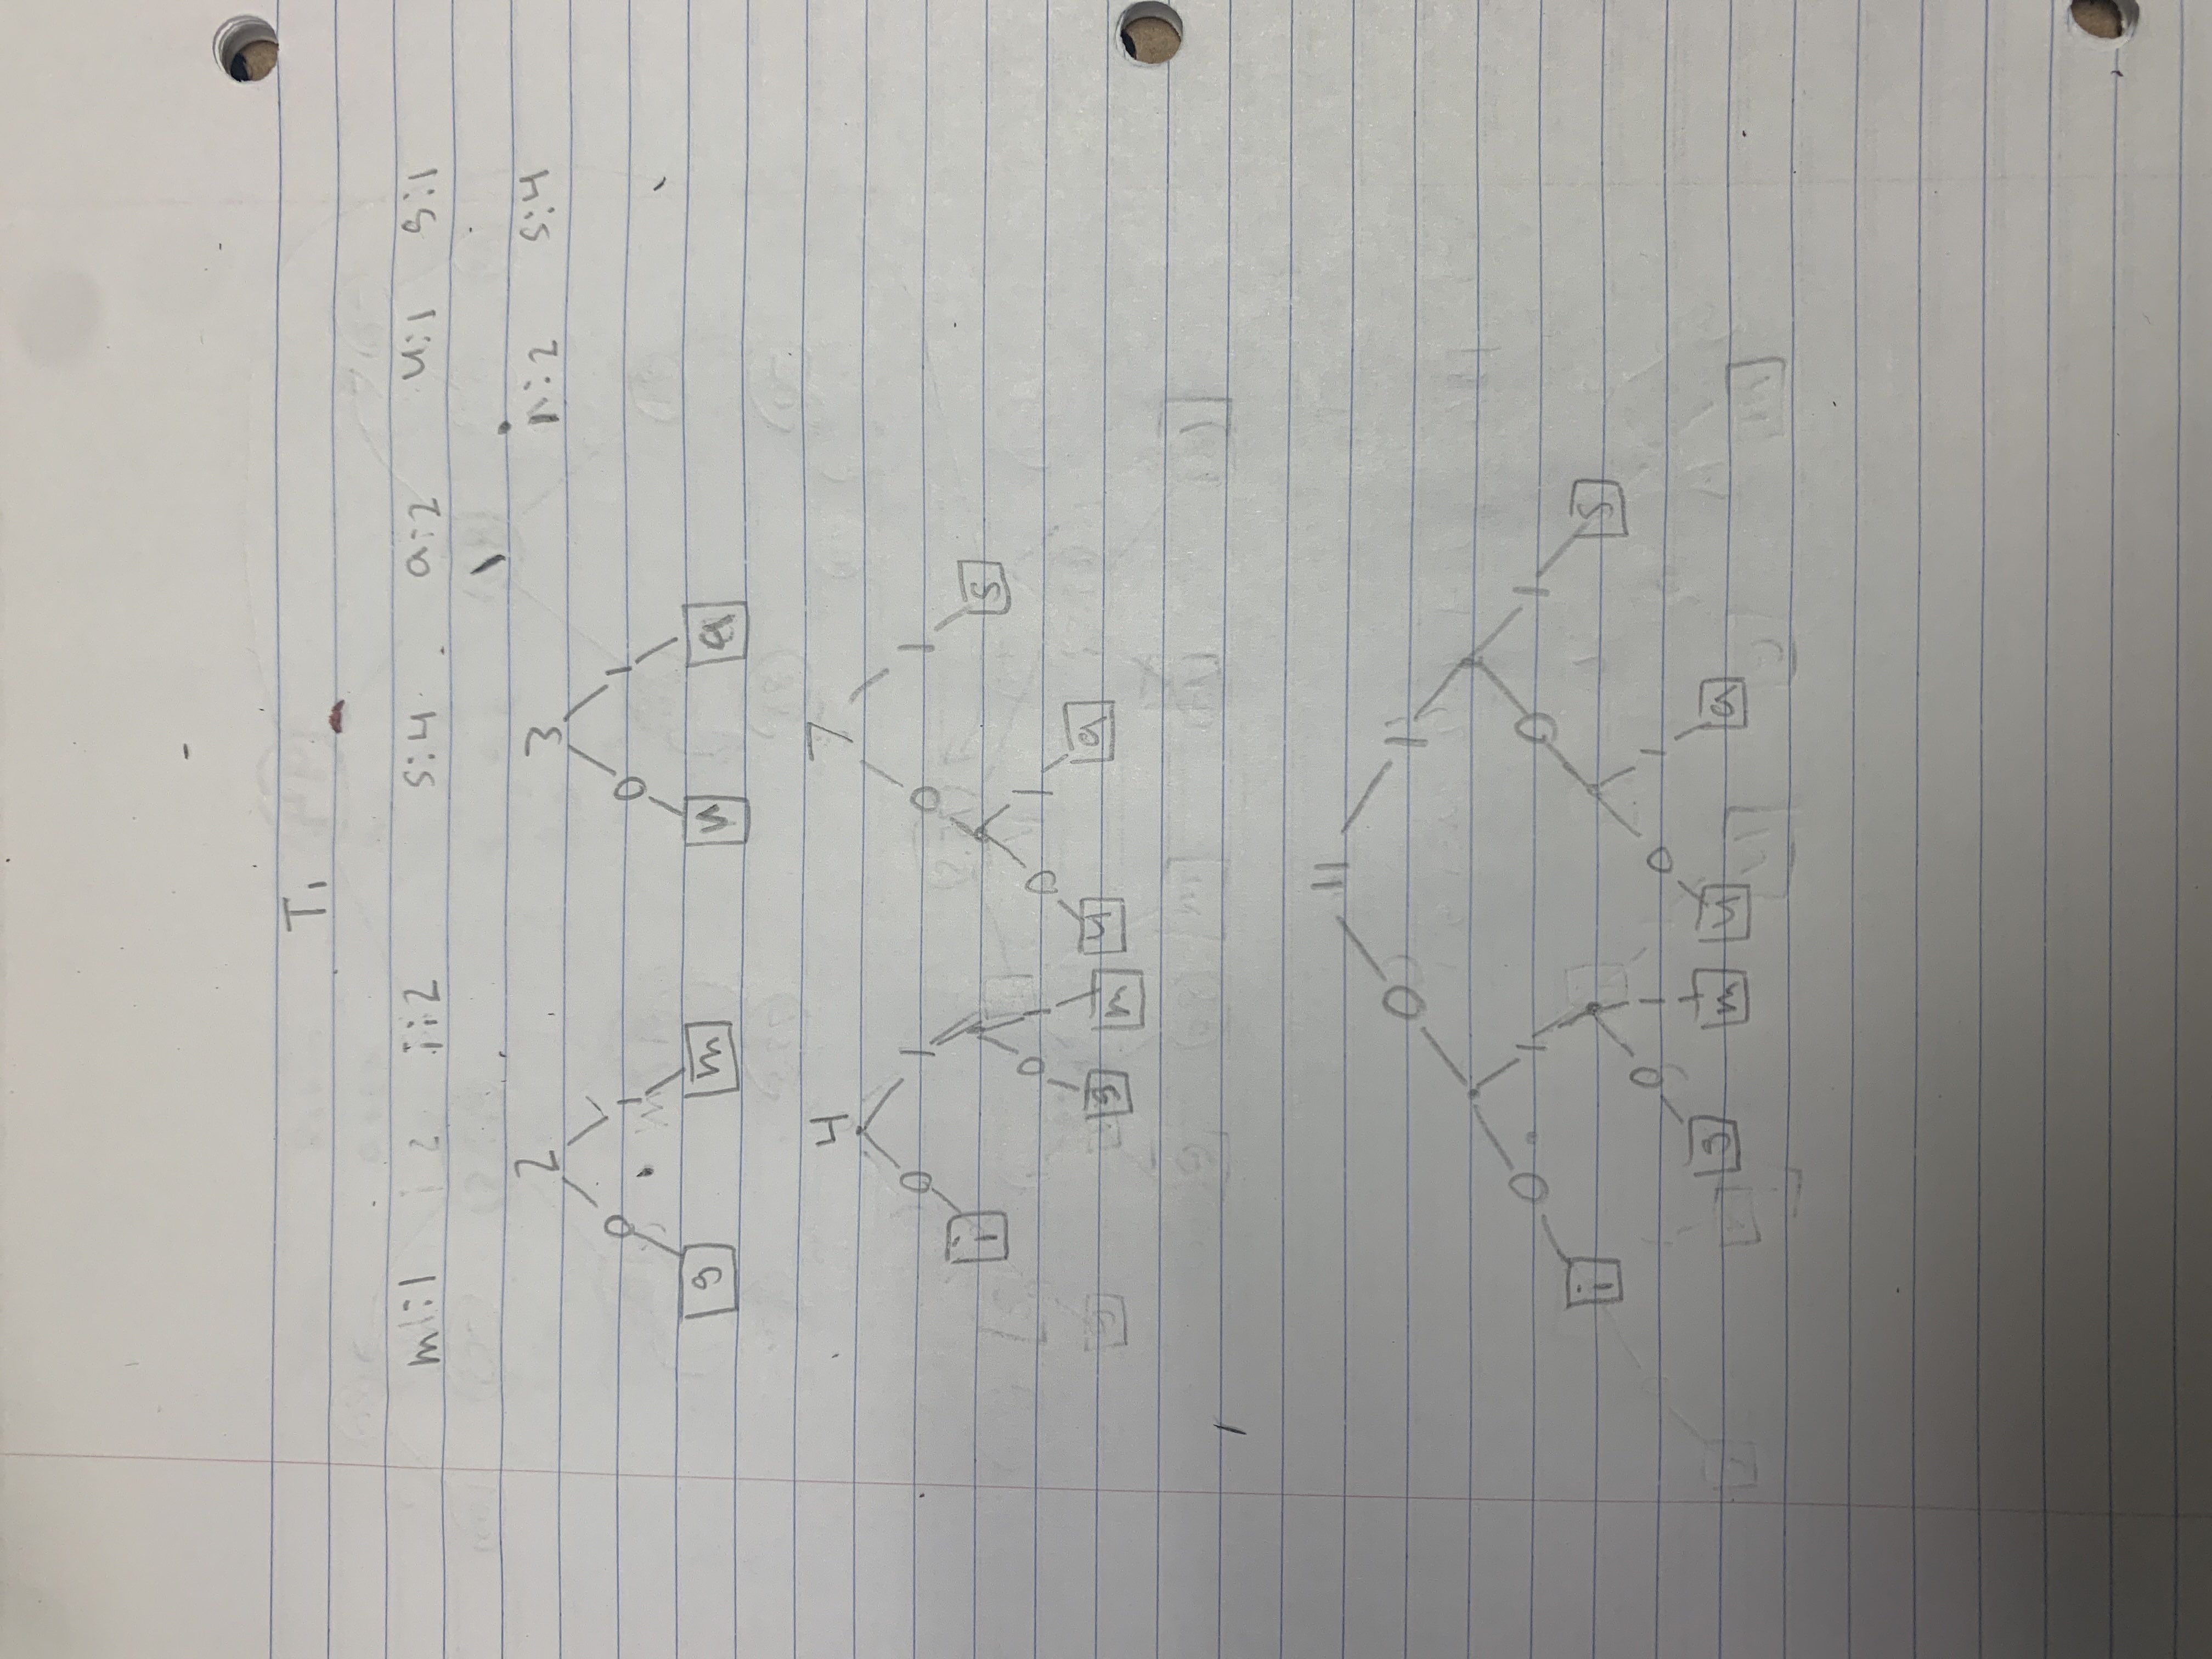
\includegraphics[width=0.8\textwidth, angle=270]{t1.jpg}
	\end{center}
	\caption{$T_1$}
	\label{figcaption}
\end{figure}
\begin{figure}[tbhp]
	\begin{center}
		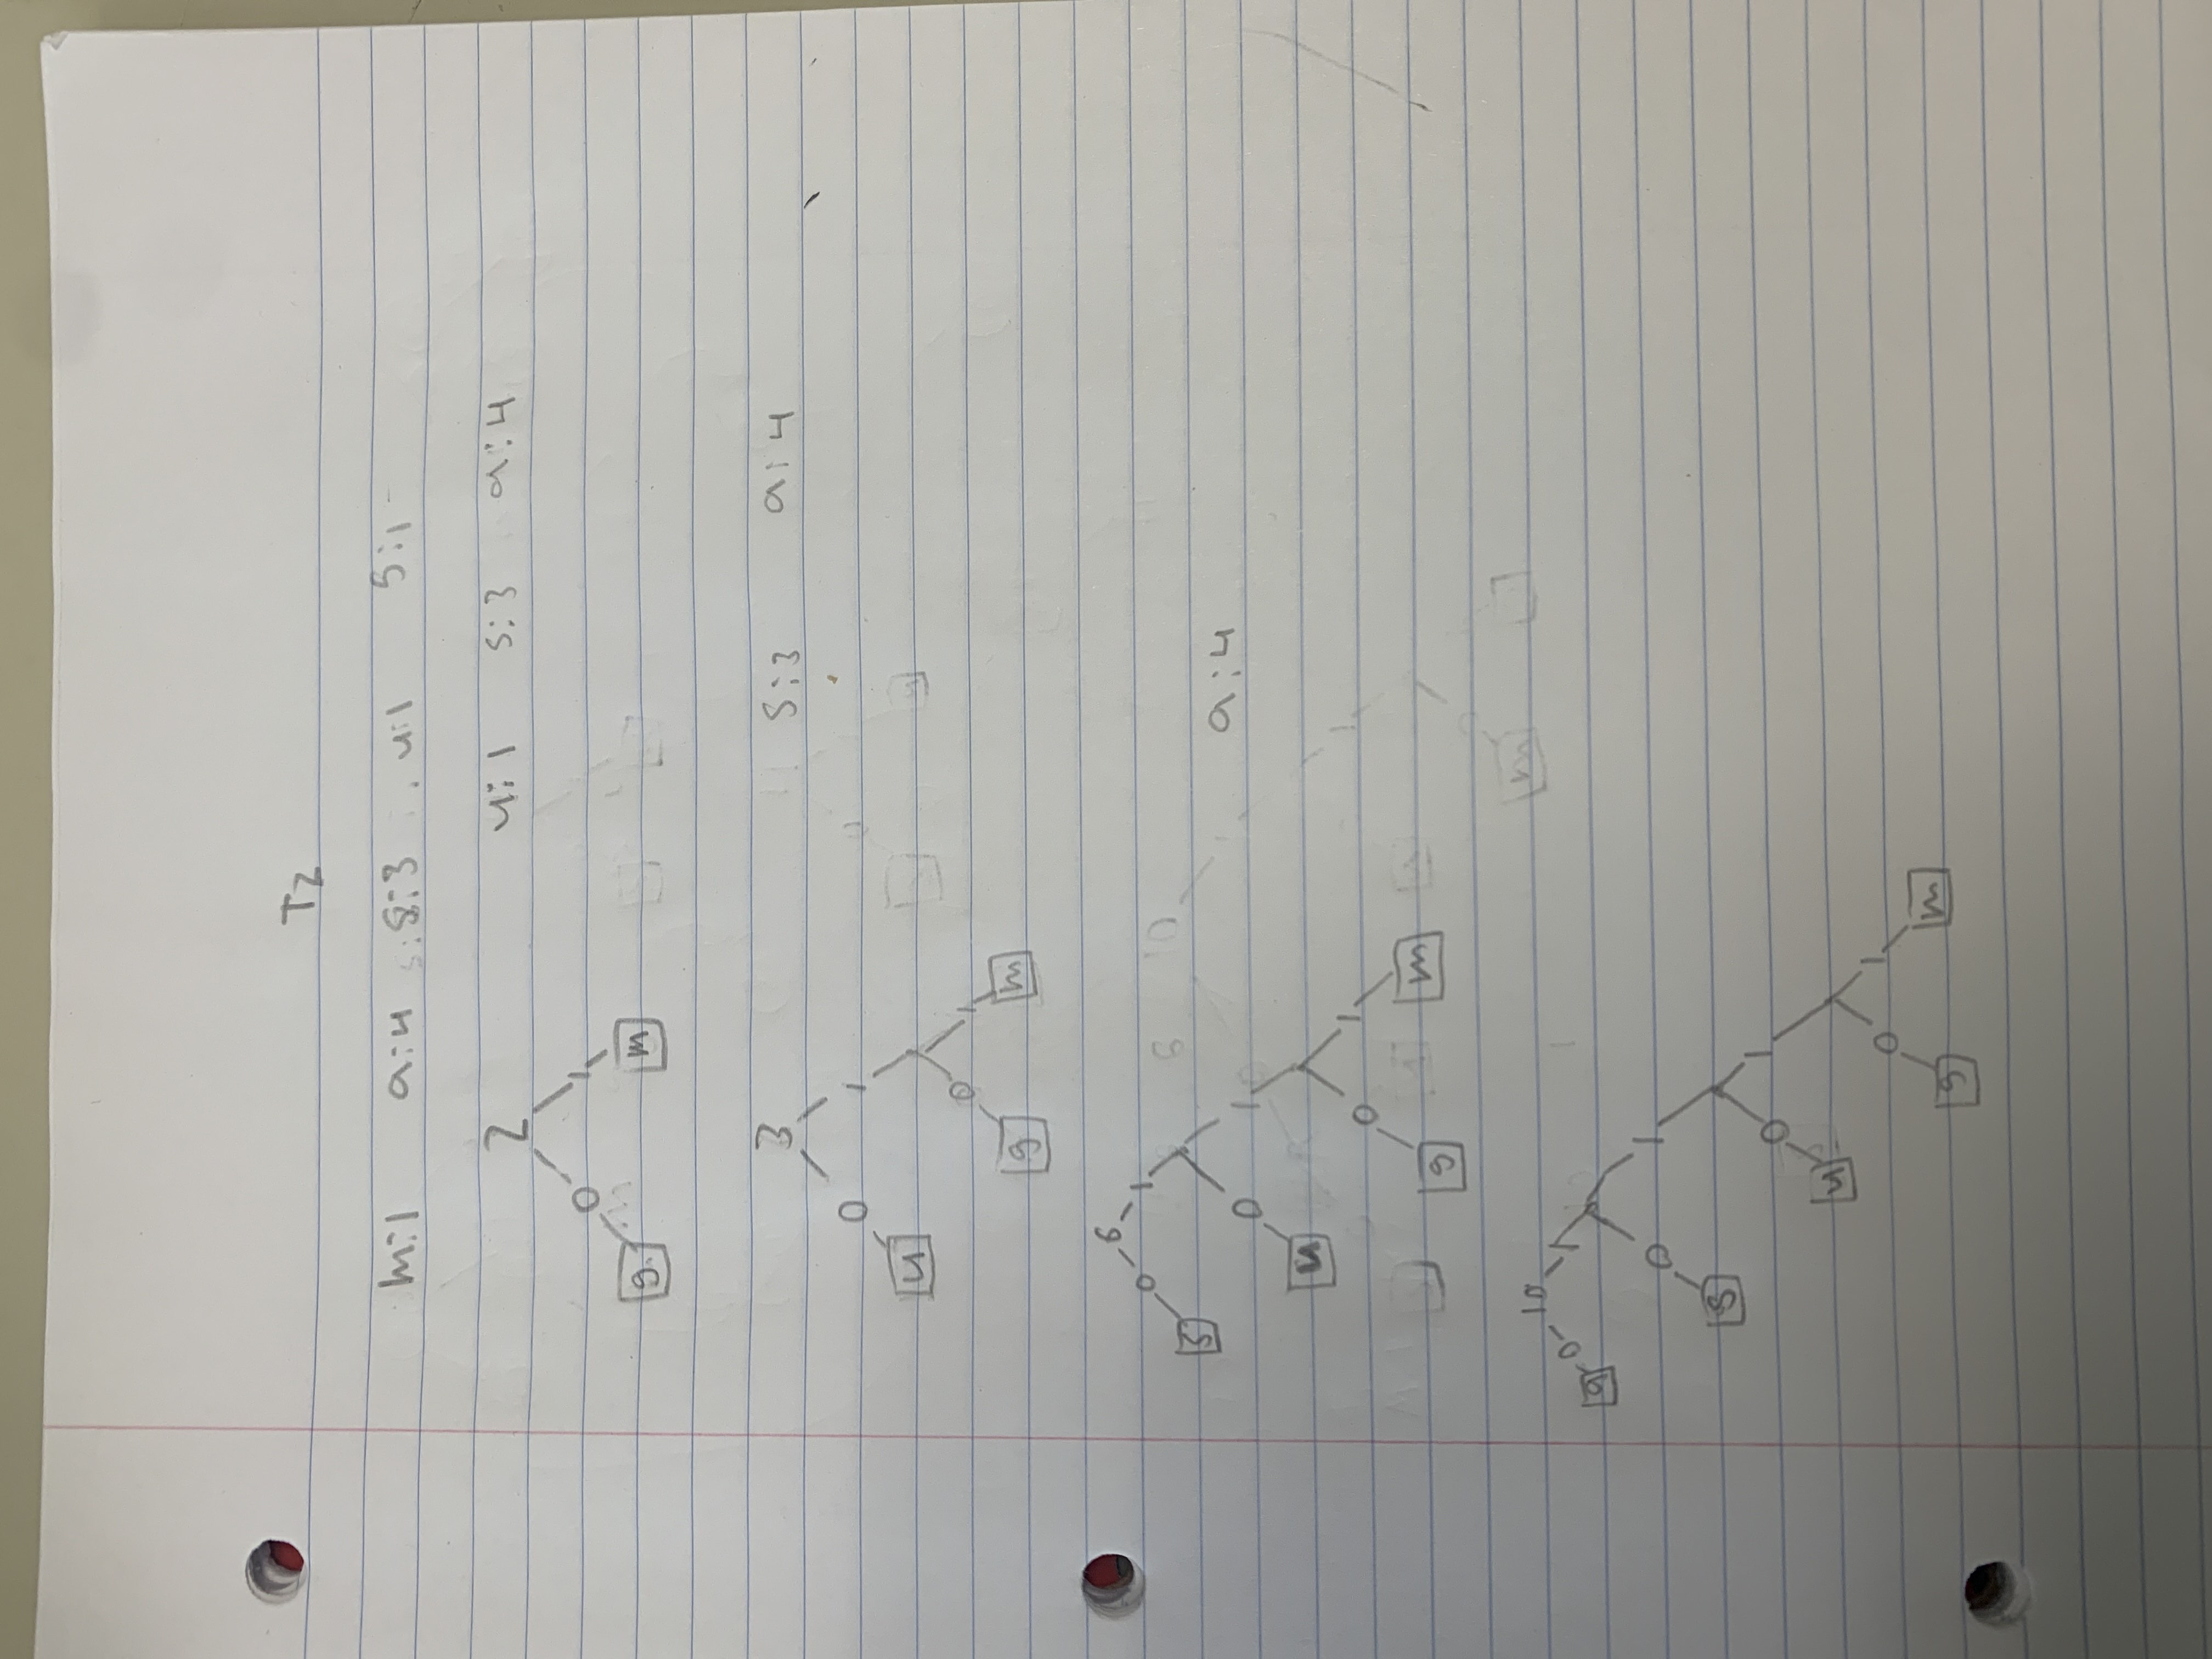
\includegraphics[width=0.8\textwidth, angle = 270]{t2.jpg}
	\end{center}
	\caption{$T_2$}
	\label{figcaption}
\end{figure}
\end{adjustwidth}
\newpage 
\begin{adjustwidth}{0em}{0pt}
\textbf{Q2b)}  Compare the compression rates of the tries from part (a) for encoding the string {\tt massasagua}.\\\\
From $T_1$ we get that the encoding for massasagua is:
\[ 011, 101, 11, 11, 101, 11, 101, 010, 100, 101 \]
The compression rate of $T_1$ is thus:
\[ \text{compression rate} : \frac{27}{10\times\lfloor\log(6)\rfloor} \approx 90\%\]
From $T_2$ we get that the encoding for massasagua is:
\[ 1111, 0, 10, 10, 0, 10, 0, 1110, 110, 0 \]
The compression rate of $T_2$ is thus:
\[ \text{compression rate} : \frac{21}{10\times\lfloor\log(5)\rfloor} \approx 70\%\]
\end{adjustwidth}
\end{document}